% !TEX root = ../../../main.tex

\chapter{Rete locale}

\section{Planimetrie}
Si riportano di seguito le planimetrie dei vari piani,comprendenti le informazioni necessarie
a stabilire la suddivisione delle postazioni di lavoro nelle relative sottoreti.

\begin{figure}[ht]
  \centering
  \begin{minipage}{.5\textwidth}
    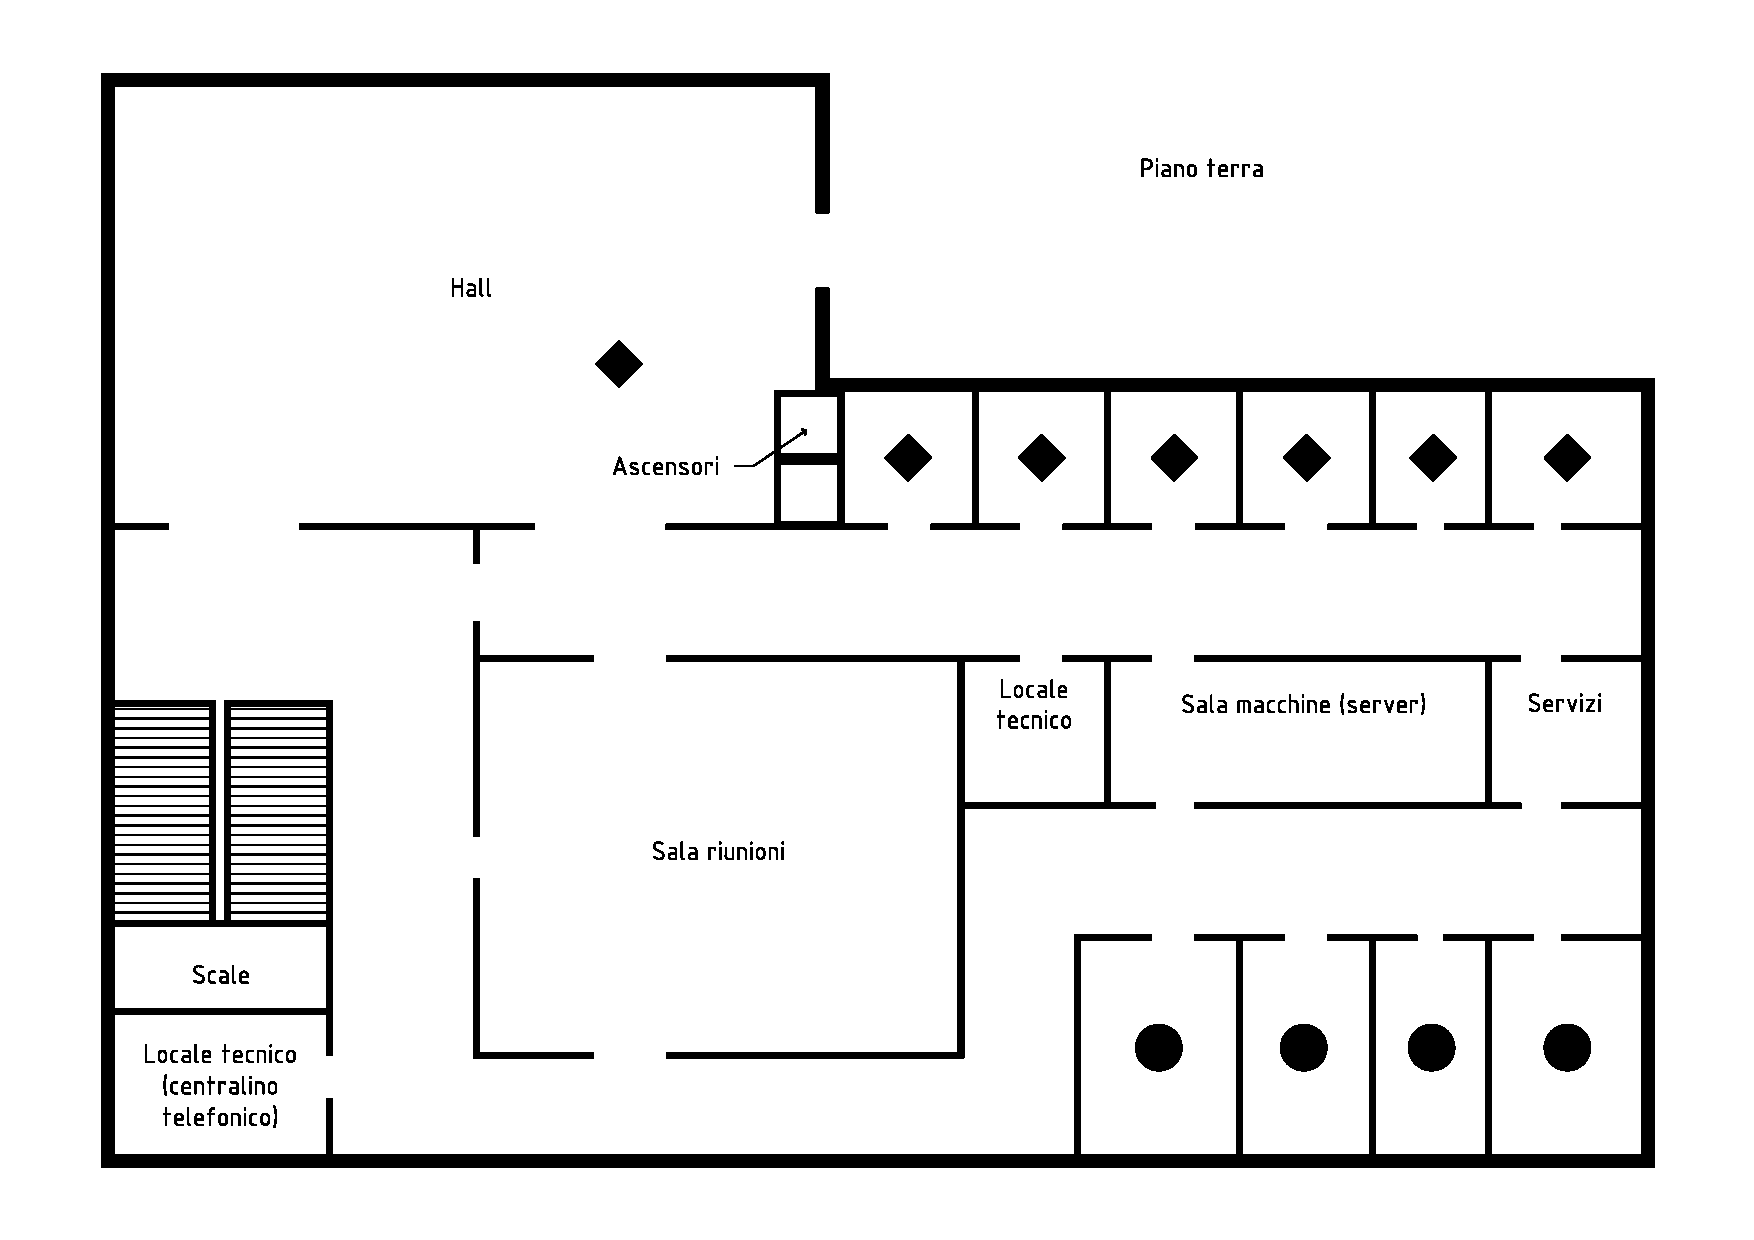
\includegraphics[width=\textwidth]{planimetrie-pianoterra-utenze}
  \end{minipage}%
  \begin{minipage}{.5\textwidth}
    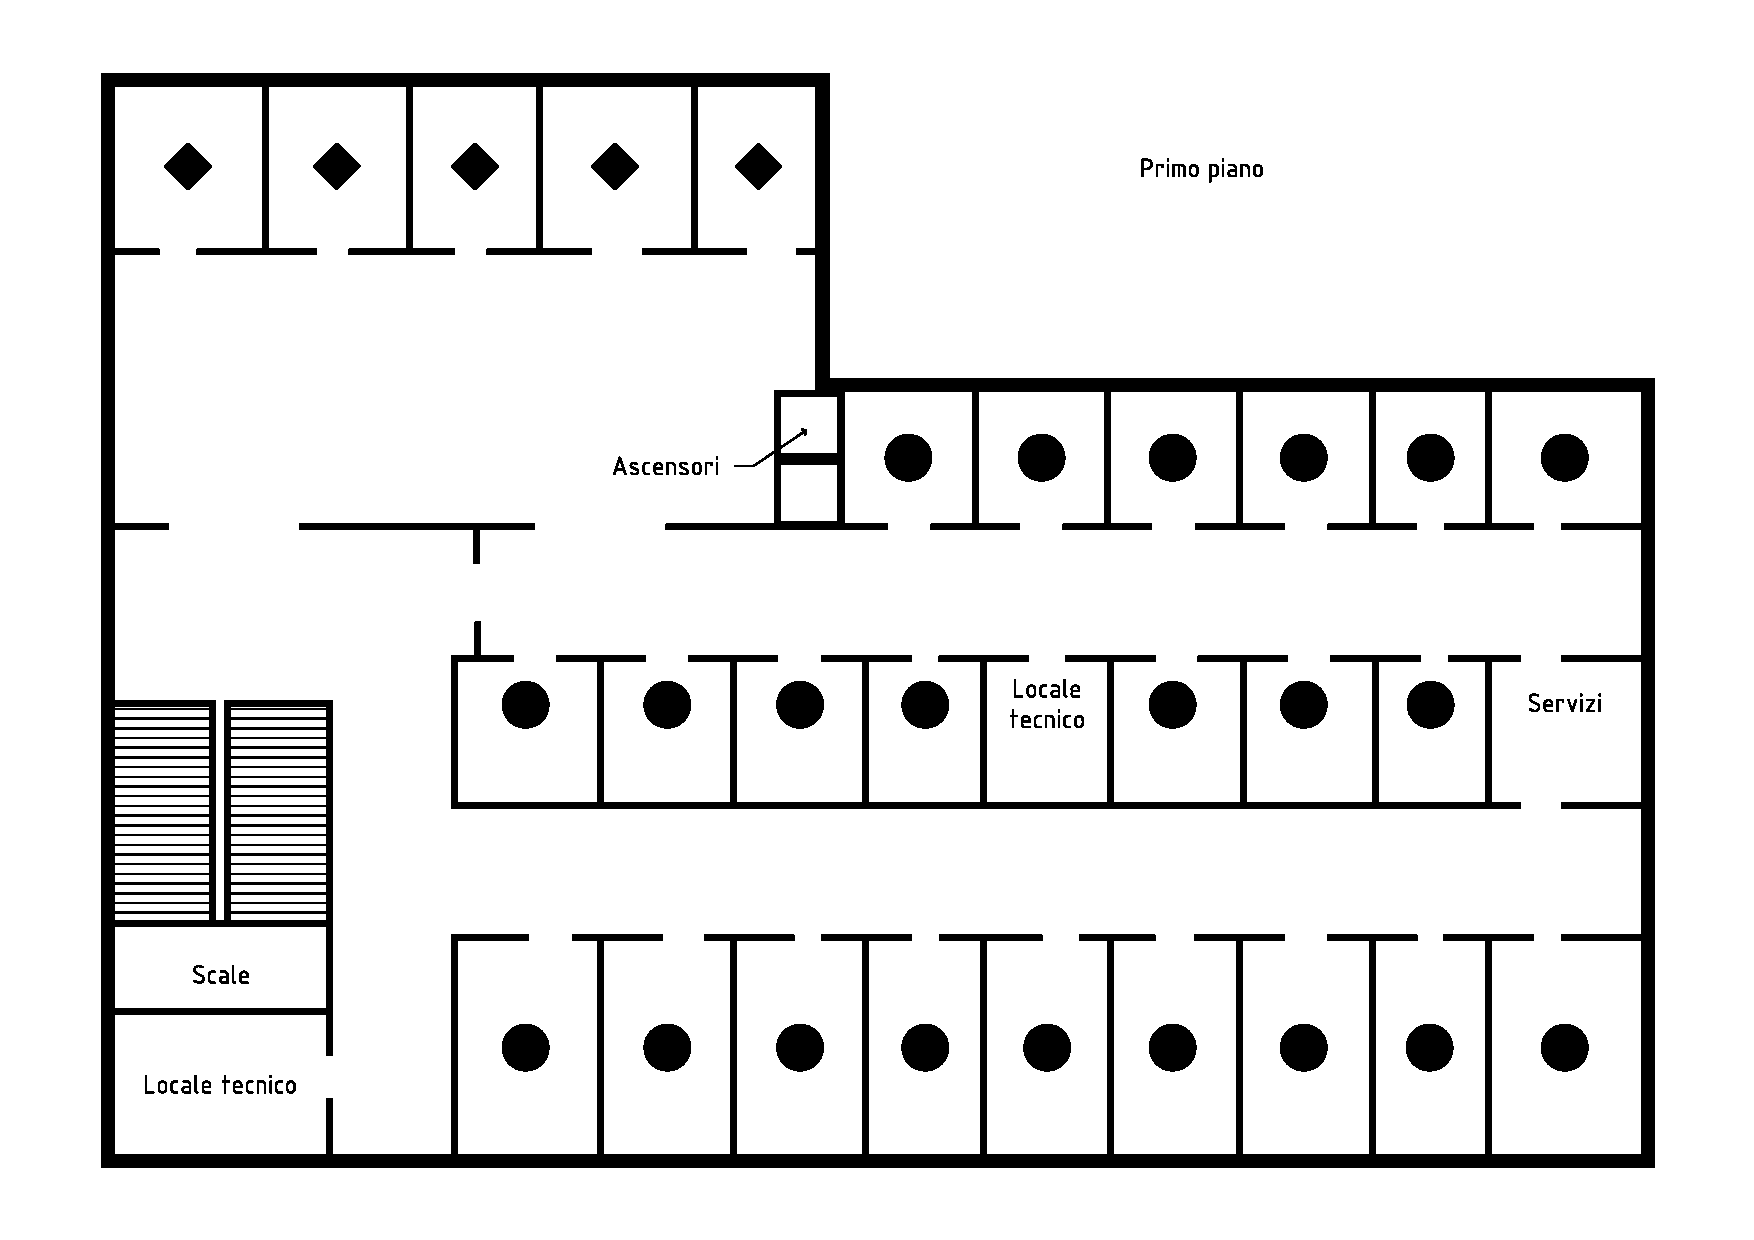
\includegraphics[width=\textwidth]{planimetrie-piano1-utenze}
  \end{minipage}
  \begin{minipage}{.5\textwidth}
    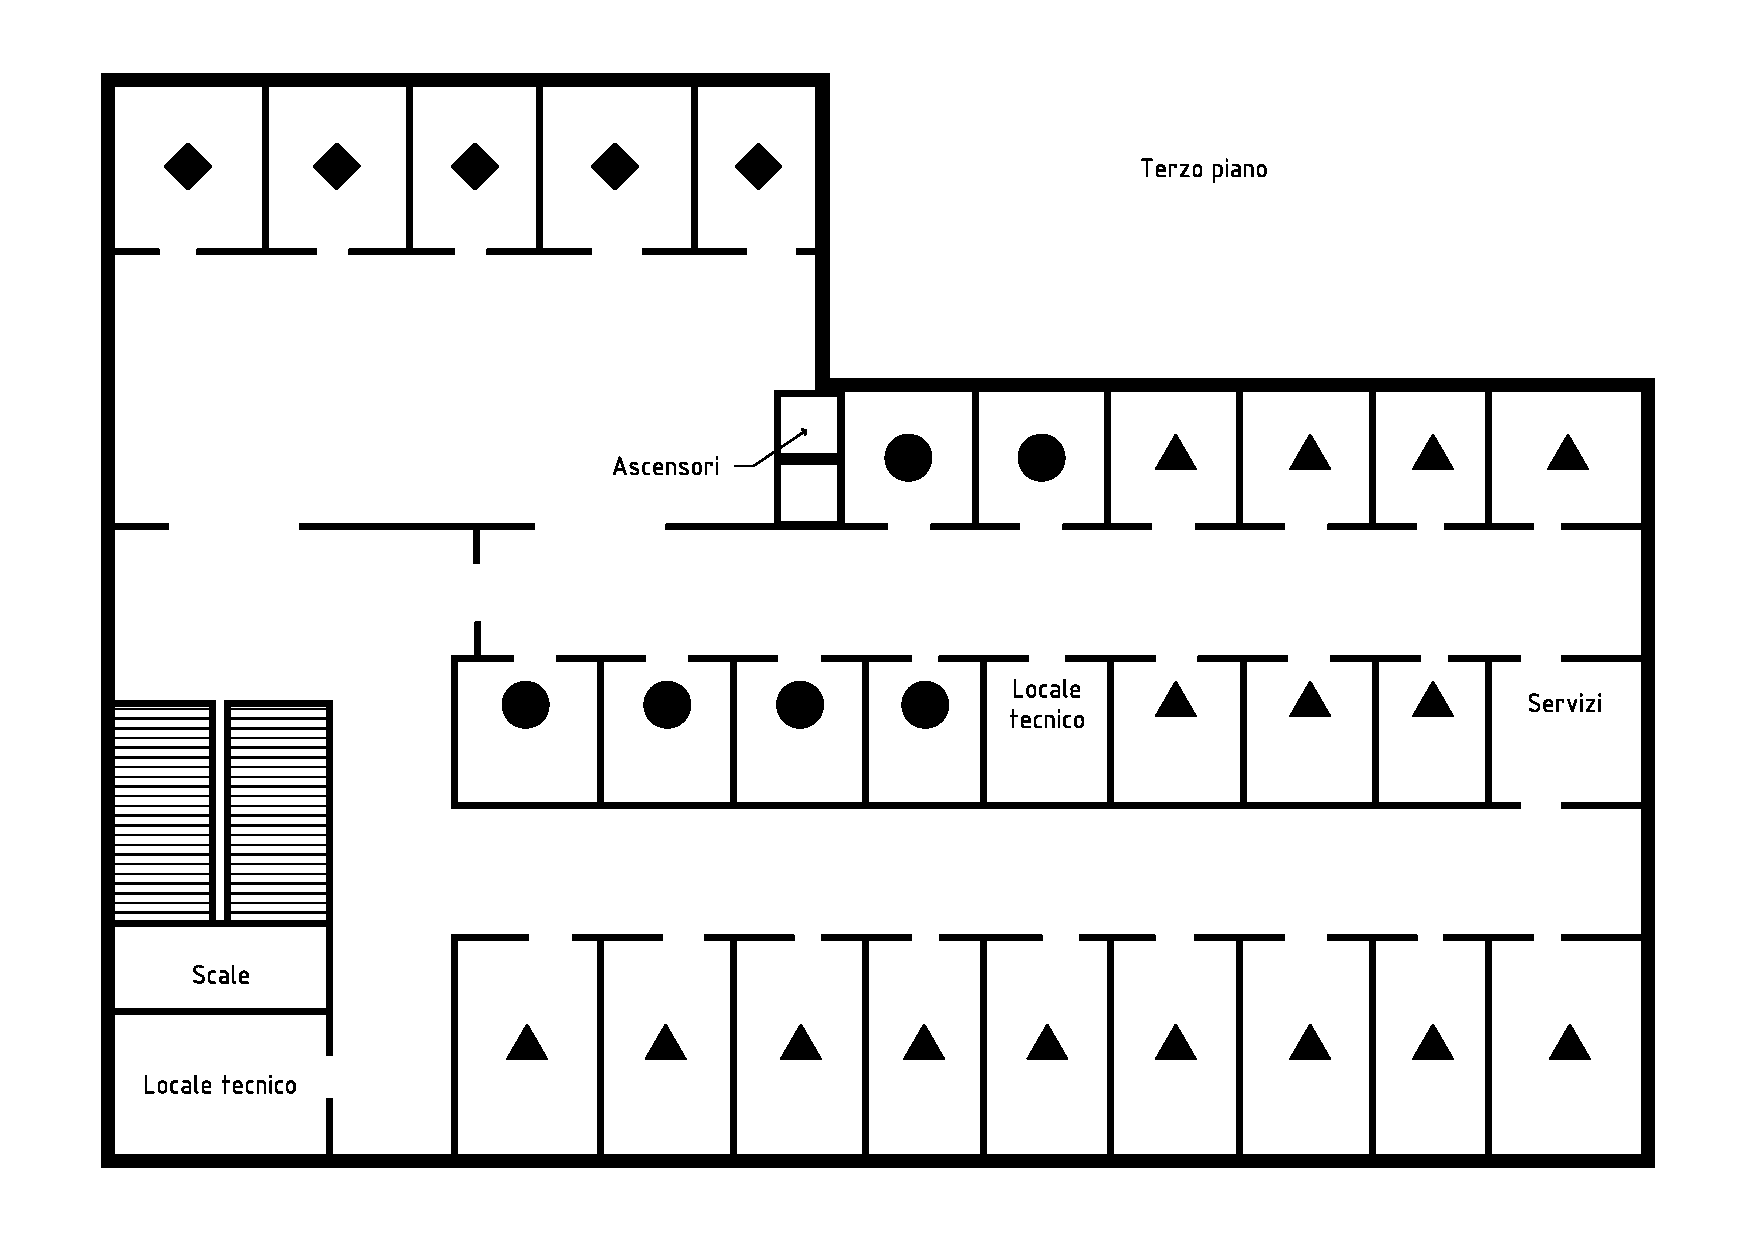
\includegraphics[width=\textwidth]{planimetrie-piano3-utenze}
  \end{minipage}
  \caption{Planimetrie con utenze.}\label{fig:planimetrie-utenze}
\end{figure}

\newpage
\section{Le sottoreti}
Ci sono tre sottoreti: la LAN di amministrazione, comprendente 28 postazioni, quella di produzione,
con 56 postazioni, ed infine quella sperimentale, da 32 utenze.

Si ritiene necessario, per motivi di sicurezza, associare alcuni dispositivi ad una rete completamente separata
rispetto a queste tre, ovvero tutti i punti in cui ci può essere un accesso condiviso ad informazioni sensibili.
Si ritiene pertanto utile isolare tutte le prese di rete presenti sul tavolo della sala riunioni insieme agli access point
per un'eventuale rete wireless per coloro che sono esterni all'azienda, in modo che, anche durante una riunione con
clienti o personale esterno (ma anche tra gruppi interni ma separati dell'azienda), non ci siano rischi per la sicurezza
delle informazioni che viaggiano sulle reti locali.

Per garantire una maggiore flessibilità a questi gruppi, si sceglie di utilizzare dispositivi di rete in grado
di creare reti LAN virtuali (VLAN).